%Correct the file name.
%X: book number
%Y: part number
%ZZZ: page number in three digits. So page 3 would be 003.

\documentclass[11pt]{amsbook}

\usepackage{../HBSuerDemir}	% ------------------------
\usepackage{graphicx}
\begin{document}

% ++++++++++++++++++++++++++++++++++++++
\hPage{b2p2/427}
% ++++++++++++++++++++++++++++++++++++++
with \\
\begin{center}
	J = 
	$\begin{vmatrix}
		a & 0 & 0 \\
		0 & b & 0   \\
		0 & 0 & c
	\end{vmatrix}$
	= abc
\end{center}
$\Rightarrow   \hAbs{V} = \int\int_{R'}\int \! abc $ $\hDif V' = abc \hAbs{R'} = abc. \frac{4}{3} \pi = \frac{4}{3}\pi abc.$
\begin{center}
	\begin{exmp} Find the volme of the solid defined by \\
		\begin{equation*}
			x^{2} + y^{2} + z^{2} \leq 16,  x^{2} + y^{2} \leq z^{2},    z \geq 0
		\end{equation*}
	\end{exmp}
\end{center}
\begin{minipage}{0.75\textwidth}
	\begin{hSolution}
		$\hAbs{R} = 4 \int_{0}^{2\sqrt{2}} \int_{0}^{\sqrt{8-x^2}} \int^{\sqrt{16-x^2-y^2}}_{\sqrt{x^2+y^2}} \hDif{z} \hDif{y} \hDif{x} $\\
		\quad Transforming it into spherical coordinates, we have the transformation
		\begin{align*}
			x=& \rho sin \varphi cos \theta \\
			y =& \rho sin \varphi sin \theta \\
			z =& \rho cos \varphi
		\end{align*}
	\end{hSolution}
\end{minipage}
\begin{minipage}{0.55\textwidth}
	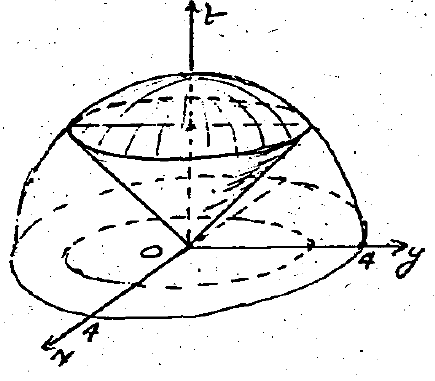
\includegraphics[width=1.0\textwidth,keepaspectratio=true]{images/b2p2-427-fig01}
\end{minipage}

with Jacobian
\begin{align*}
	J=& \frac{\partial(x,y,z)}{\partial(\theta,\varphi,\rho)} \\
	=& 
	\begin{vmatrix}
		-\rho \sin\varphi \sin\theta & \rho \cos \varphi \cos \theta & \sin \varphi \cos \theta \\
		\rho \sin \varphi \cos \theta & \rho \cos \varphi \sin \theta & \sin \varphi \sin \theta \\
		0 & - \rho \sin \varphi & cos \varphi
	\end{vmatrix}
	= - \rho^2 \sin\varphi \\
	\hAbs{R} =& 4 \int^{\pi/2}_0 \int^{\pi/4}_{0} \int^4_{0} \rho^2 \sin \varphi. \hDif{\rho} \hDif{\varphi} \hDif{\theta}  = \frac{16}{3} \sqrt{2} \pi
\end{align*}




% =======================================
%\section{aaaah}

%u




% =======================================
%\subsection{bbb}





% =======================================
%\subsubsection

%This is the first figure. 
%\begin{figure}[htb]
%	\centering
%	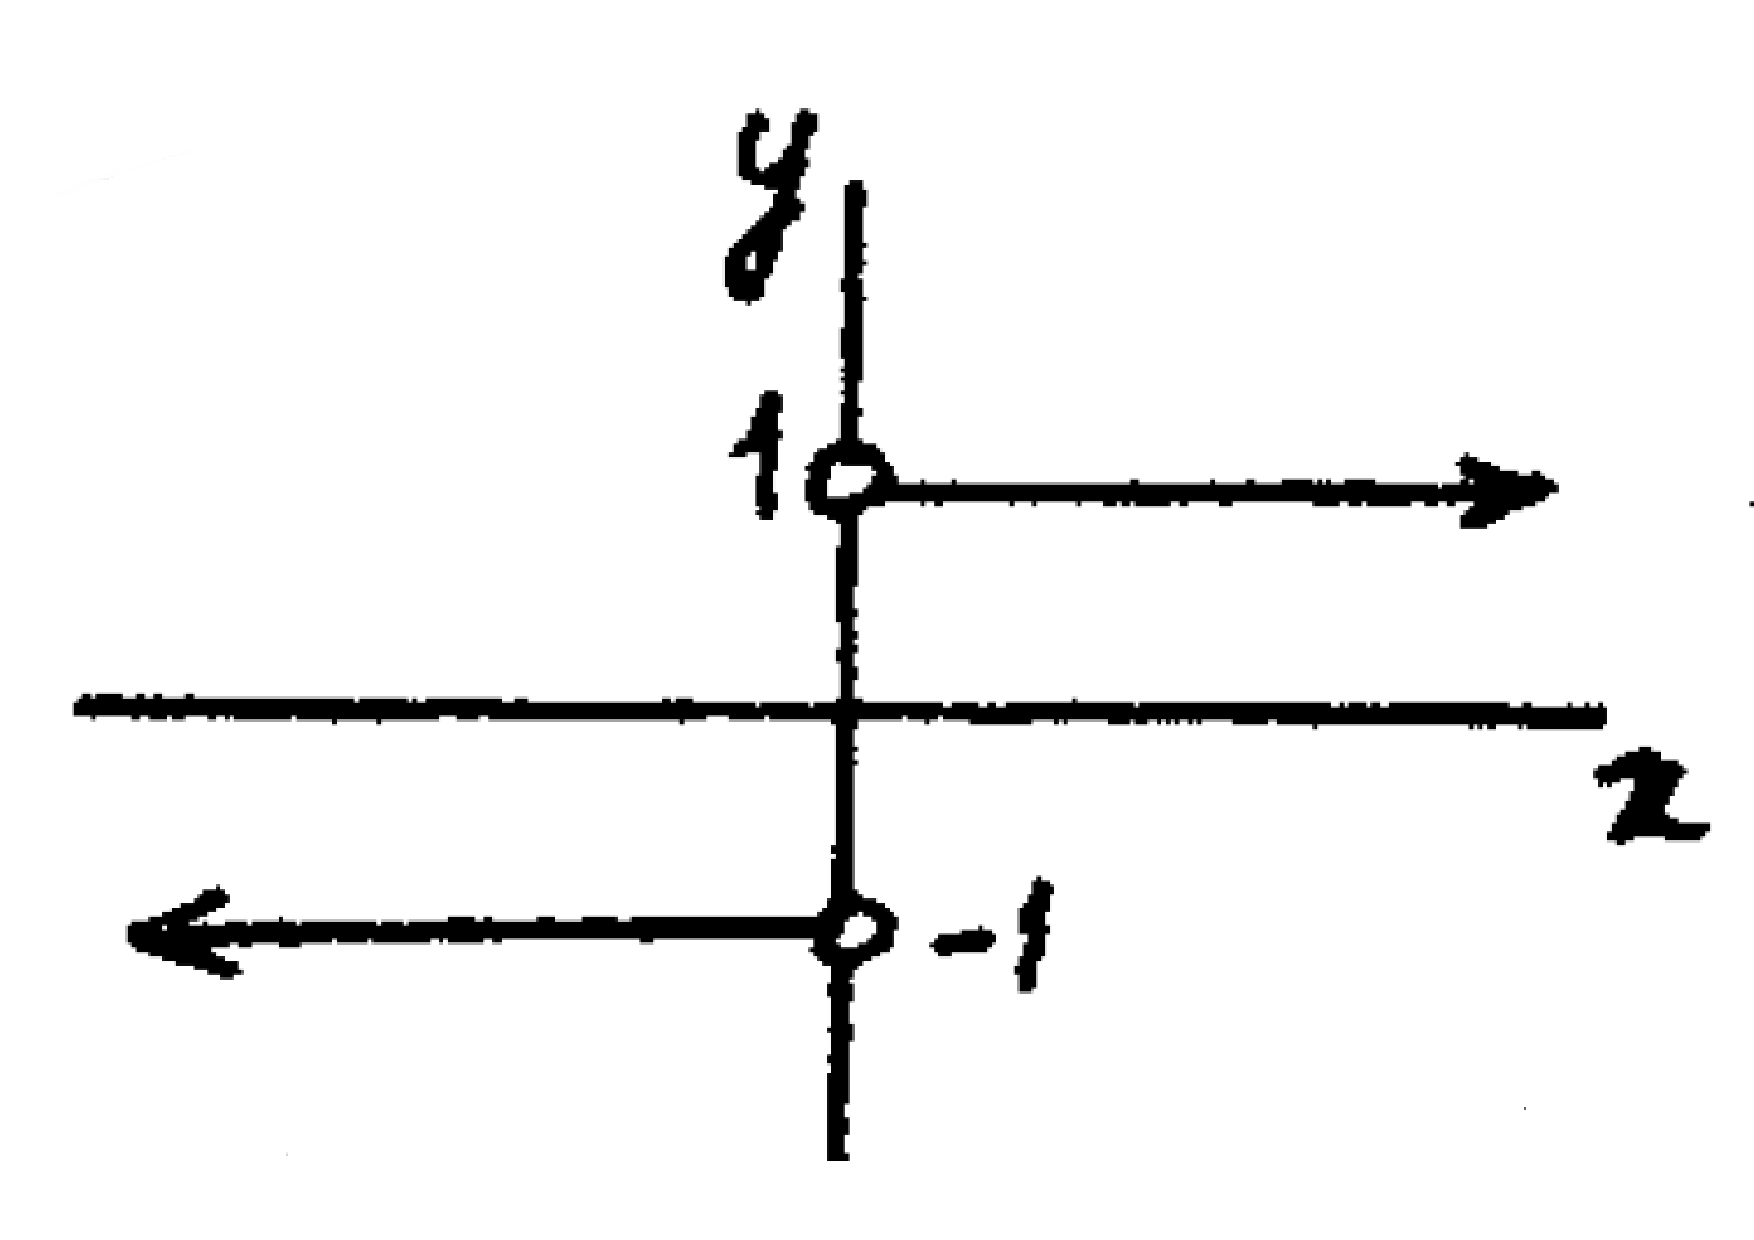
\includegraphics[width=0.45\textwidth]{images/bXpY-ZZZ-fig01}
%	\caption{Classification of complex numbers}
%	\label{fig:classificationOfComplexNumbersA}
%\end{figure}
%This is the second figure
%\begin{figure}[htb]
%	\centering
%	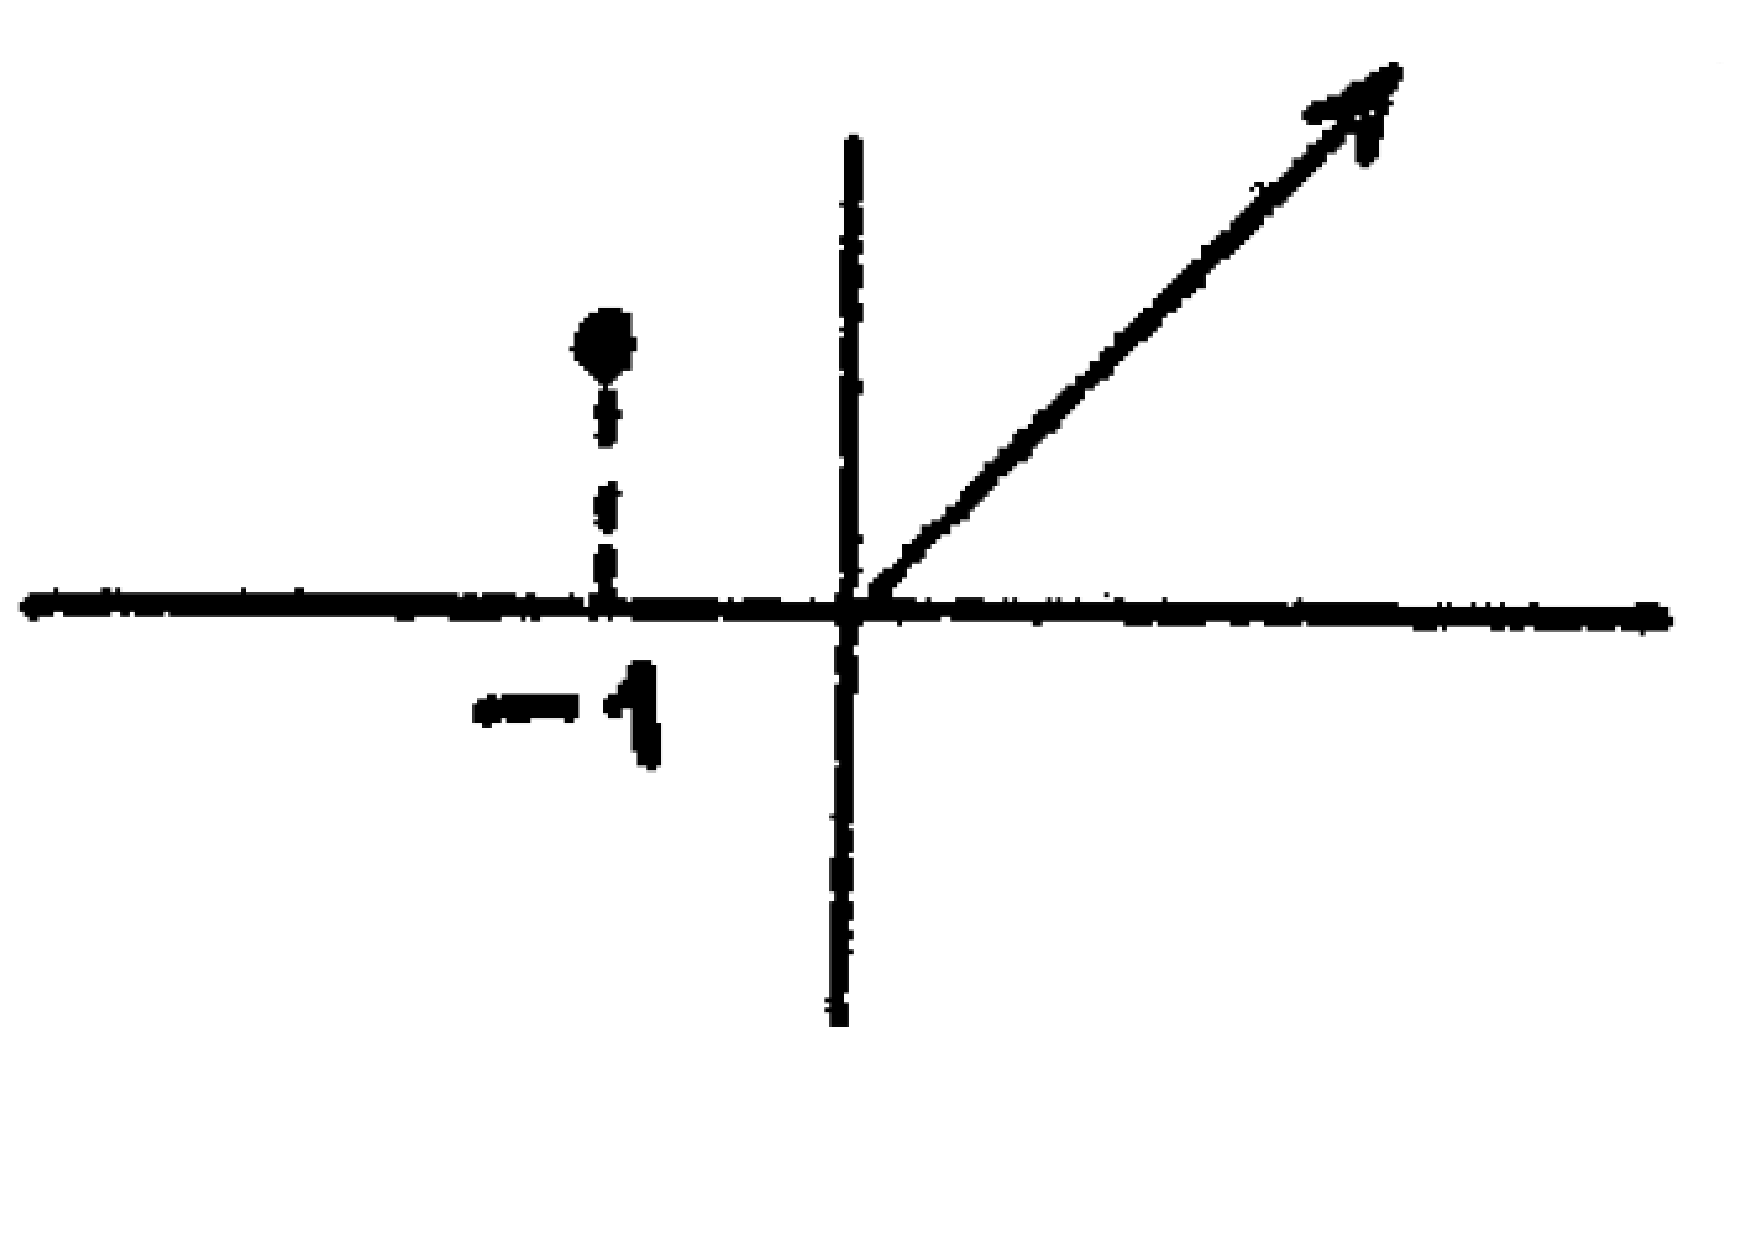
\includegraphics[width=0.45\textwidth]{images/bXpY-ZZZ-fig02}
%	\caption{Classification of complex numbers}
%	\label{fig:classificationOfComplexNumbersA}
%\end{figure}






% =======================================================
\end{document}  

%==== templates ====

%==== environments ====

%\begin{figure}[htb]
%	\centering
%	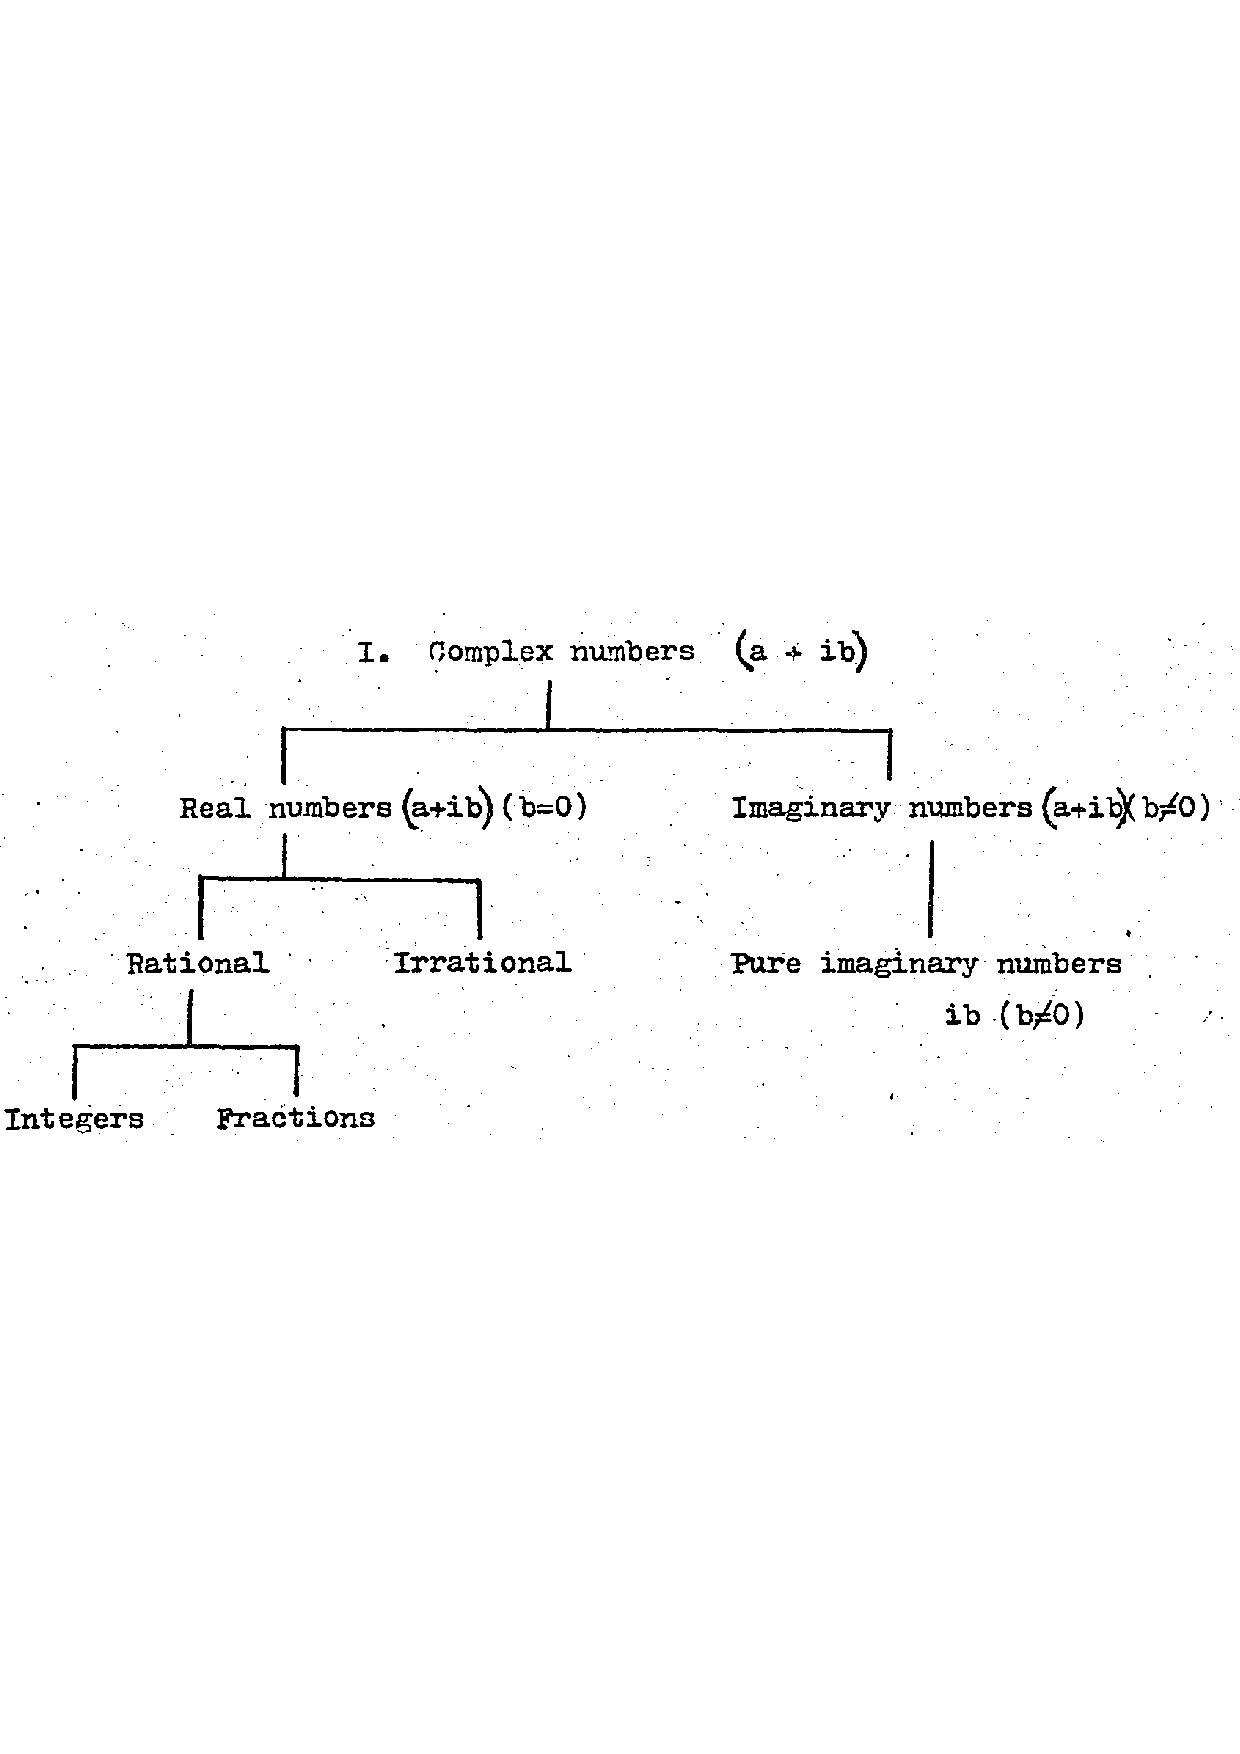
\includegraphics[width=0.9\textwidth]{images/SD-1-1p15A}
%	\caption{Classification of complex numbers}
%	\label{fig:classificationOfComplexNumbersA}
%\end{figure}

%\begin{center}
%\begin{tabular}{cc}
%\end{tabular}
%\end{center}

%\begin{exmp}
%\begin{hSolution}
%\end{hSolution}
%\end{exmp}

%\begin{hEnumerateAlpha}
%\end{hEnumerateAlpha}

%\begin{hEnumerateRoman}
%\end{hEnumerateRoman}

%$
%\begin{bmatrix}
%\end{bmatrix}
%$

%\frac{aaaa}{bbb}
%\frac{a_{n}}{b_{n}}
%\left( aaaa \right)
%\Longrightarrow

%\begin{multicols}{2}
%	bb
%\columnbreak
%	aa
%\end{multicols}
